\documentclass[../main.tex]{subfiles}

\addbibresource{\subfix{../references.bib}}

\begin{document}

\ifSubfilesClassLoaded{%
    \setcounter{chapter}{9}%
    \begin{refsection}
}{}

\chapter{Runtime Environment dan Memory Management}
\label{chap:runtime-environment}

\begin{subcpmk}
  \item \textbf{Sub-CPMK 5.1:} Mendesain runtime environment untuk bahasa pemrograman
\end{subcpmk}

% ============================================================
% MATERI POKOK
% ============================================================
\section{Layout Memori dan Segmentasi}

\compiler{Runtime Environment} mengelola bagaimana program menggunakan memori saat dieksekusi. Manajemen memori saat runtime merupakan salah satu aspek yang paling krusial dalam performa dan keamanan sebuah program hasil kompilasi \cite{ucsd2024compiler}.

\subsection{Segmen Memori Utama}
\begin{itemize}
    \item \textbf{Text/Code Segment}: Menyimpan instruksi biner hasil kompilasi. Biasanya bersifat \textit{read-only}.
    \item \textbf{Data Segment}: Menyimpan variabel global dan statis yang sudah diinisialisasi.
    \item \textbf{Stack}: Segmen yang tumbuh ke bawah untuk mengelola pemanggilan fungsi dan variabel lokal.
    \item \textbf{Heap}: Segmen yang tumbuh ke atas untuk alokasi memori dinamis (\textit{runtime allocation}).
\end{itemize}

\begin{figure}[!htbp]
    \centering
    \adjustbox{max width=0.6\textwidth,center}{%
    \begin{tikzpicture}[
        seg/.style={rectangle, draw=blue!50, fill=blue!10, text width=3cm, minimum height=0.6cm, font=\tiny, align=center}
    ]
    \node[seg] (s) {Stack (↓)};
    \node[seg, below=1cm of s] (h) {Heap (↑)};
    \node[seg, below=0.2cm of h] (d) {Data};
    \node[seg, below=0.2cm of d] (t) {Text};
    \end{tikzpicture}%
    }
    \caption{Model konseptual organisasi memori runtime}
\end{figure}

\section{Activation Records dan Skoping Bertingkat}

Setiap kali sebuah fungsi dipanggil, struktur data yang disebut \compiler{Activation Record} (atau \textit{Stack Frame}) dibuat di puncak stack untuk mengelola eksekusi fungsi tersebut.

\subsection{Struktur Stack Frame}
Sebuah stack frame biasanya menampung informasi kritis berikut:
\begin{enumerate}
    \item \textbf{Return Address}: Alamat instruksi berikutnya di \textit{caller} yang harus dieksekusi setelah fungsi selesai.
    \item \textbf{Control Link (Dynamic Link)}: Pointer ke stack frame milik fungsi pemanggil (\textit{caller}). Digunakan untuk menghapus frame saat ini dan kembali ke frame sebelumnya.
    \item \textbf{Access Link (Static Link)}: Pointer ke stack frame milik fungsi yang secara leksikal (sintaksis) membungkus fungsi saat ini. Digunakan untuk mengakses variabel non-lokal dalam bahasa yang mendukung fungsi bersarang (\textit{nested functions}).
    \item \textbf{Saved Registers}: Nilai register prosesor yang harus dipulihkan sebelum kembali.
    \item \textbf{Local Variables}: Ruang untuk data yang dideklarasikan di dalam fungsi tersebut.
\end{enumerate}

\subsection{Menangani Akses Variabel Non-Lokal}
Dalam bahasa seperti Pascal atau Python, fungsi di dalam fungsi dapat mengakses variabel milik induknya. Ada dua teknik utama untuk mengelola ini:
\begin{enumerate}
    \item \textbf{Access Links}: Membentuk rantai pointer statis. Jika variabel berada di tingkat bersarang ke-3 di atasnya, kompilator harus mengikuti rantai link tersebut 3 kali. Ini sederhana tapi lambat jika nesting terlalu dalam.
    \item \textbf{Displays}: Menggunakan larik (\textit{array}) global berisi pointer ke frame yang sedang aktif di setiap tingkat bersarang. Dengan \textit{display}, akses ke tingkat mana pun selalu berbiaya konstan (satu kali akses larik).
\end{enumerate}

\begin{figure}[!htbp]
    \centering
    \adjustbox{max width=0.8\textwidth,center}{%
    \begin{tikzpicture}[
        node/.style={rectangle, draw=blue!50, fill=blue!10, text width=3cm, minimum height=0.6cm, font=\tiny, align=center}
    ]
    \node[node] (f1) {Frame A (Outer)};
    \node[node, below=0.5cm of f1] (f2) {Frame B (Inner)};
    \draw[->, >=stealth, bend left=45, blue, dashed] (f2.east) to node[right, font=\tiny] {Access Link} (f1.east);
    \draw[->, >=stealth, bend right=45, red] (f2.west) to node[left, font=\tiny] {Control Link} (f1.west);
    \end{tikzpicture}%
    }
    \caption{Perbedaan Aliran Control Link (Dinamis) vs Access Link (Statis)}
\end{figure}

\section{Mekanisme Panggilan: Konvensi Register}

Prosedur pemanggilan fungsi melibatkan pembagian tanggung jawab antara fungsi yang memanggil (\textit{caller}) dan fungsi yang dipanggil (\textit{callee}) dalam mengelola register CPU.

\subsection{Caller-Saved vs Callee-Saved}
Kompilator menggunakan konvensi berikut untuk menjaga integritas data:
\begin{enumerate}
    \item \textbf{Caller-Saved Registers} (Volatile): Register yang nilainya boleh dirusak oleh fungsi yang dipanggil. Jika \textit{caller} membutuhkan nilai di register ini setelah panggilan fungsi, \textit{caller} harus menyimpannya ke stack sebelum perintah \code{call}. Contoh pada x86-64: \texttt{rax}, \texttt{rcx}, \texttt{rdx}.
    \item \textbf{Callee-Saved Registers} (Non-volatile): Register yang nilainya harus tetap sama bagi \textit{caller} sebelum dan sesudah panggilan. Jika \textit{callee} ingin menggunakan register ini, ia harus menyimpan isinya di awal fungsi (\textit{prologue}) dan memulihkannya di akhir fungsi (\textit{epilogue}). Contoh pada x86-64: \texttt{rbx}, \texttt{rbp}, \texttt{r12-r15}.
\end{enumerate}

\subsection{Penyaluran Parameter}
Pada arsitektur modern (seperti System V AMD64 ABI), enam parameter pertama biasanya dikirim melalui register (\texttt{rdi, rsi, rdx, rcx, r8, r9}) alih-alih stack untuk meningkatkan performa. Parameter ke-7 dan seterusnya baru dikirim melalui stack.

\begin{figure}[!htbp]
    \centering
    \adjustbox{max width=0.8\textwidth,center}{%
    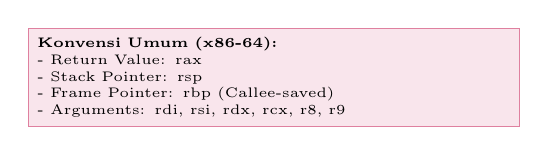
\begin{tikzpicture}[
        rect/.style={rectangle, draw=purple!50, fill=purple!10, text width=6cm, font=\tiny}
    ]
    \node[rect] (reg) {
        \textbf{Konvensi Umum (x86-64):}\\
        - Return Value: \code{rax}\\
        - Stack Pointer: \code{rsp}\\
        - Frame Pointer: \code{rbp} (Callee-saved)\\
        - Arguments: rdi, rsi, rdx, rcx, r8, r9
    };
    \end{tikzpicture}%
    }
    \caption{Peta Penggunaan Register dalam Prosedur Panggilan}
\end{figure}

\section{Manajemen Dinamis dan Strategi Heap}

Berbeda dengan stack yang memiliki struktur kaku, \compiler{Heap} adalah area memori bebas di mana blok-blok dapat dialokasikan dan dibebaskan dalam urutan apa pun.

\subsection{Strategi Alokasi Pemuatan}
Kompilator dan pustaka runtime menggunakan algoritma tertentu untuk mencari blok kosong yang cukup besar:
\begin{enumerate}
    \item \textbf{First-Fit}: Mencari dari awal heap dan mengambil blok kosong pertama yang ukurannya cukup. Algoritma ini sangat cepat namun cenderung meninggalkan fragmentasi di awal heap.
    \item \textbf{Best-Fit}: Mencari ke seluruh heap untuk menemukan blok kosong terkecil yang masih cukup menampung permintaan. Ini meminimalkan sisa ruang (\textit{leftover}) namun pencariannya lambat.
    \item \textbf{Next-Fit}: Mirip First-fit, tapi pencarian dimulai dari titik terakhir alokasi dilakukan. Ini mendistribusikan alokasi lebih merata di seluruh heap.
\end{enumerate}

\subsection{Masalah Fragmentasi}
Tujuan utama pengelola memori adalah menekan \textbf{External Fragmentation} (adanya banyak lubang kecil yang terpisah-pisah sehingga tidak bisa melayani alokasi satu blok besar). Solusinya adalah \textit{Coalescing} (menggabungkan blok kosong yang bertetangga menjadi satu) atau \textit{Compaction} (menggeser blok-blok yang terisi ke satu sisi).

\begin{figure}[!htbp]
    \centering
    \adjustbox{max width=0.8\textwidth,center}{%
    \begin{tikzpicture}[
        block/.style={rectangle, draw, minimum width=1cm, minimum height=0.5cm, font=\tiny}
    ]
    \node[block, fill=blue!20] (b1) {Used};
    \node[block, right=0pt of b1] (f1) {Free};
    \node[block, right=0pt of f1, fill=blue!20] (b2) {Used};
    \node[block, right=0pt of b2] (f2) {Free};
    \node[below=0.2cm of f1, font=\tiny] {Lubang Fragmentasi};
    \end{tikzpicture}%
    }
    \caption{Ilustrasi Fragmentasi Eksternal pada Heap}
\end{figure}

\section{Praktikum: Simulator Runtime Stack}

Mahasiswa akan mempelajari cara kerja stack frame melalui implementasi simulator sederhana. Simulator ini melacak pembuatan dan penghapusan \textit{Activation Record} setiap kali ada simulasi pemanggilan fungsi.

\begin{lstlisting}[language=C++]
struct Frame {
    string funcName;
    Frame* caller;
    map<string, int> locals;
};

class StackSimulator {
    Frame* top = nullptr;
public:
    void call(string name) {
        top = new Frame{name, top};
    }
    void returnFunc() {
        Frame* old = top;
        top = top->caller;
        delete old;
    }
};
\end{lstlisting}
Simulator ini membantu memvisualisasikan bagaimana variabel lokal diisolasi antar fungsi dan bagaimana rekursi dapat menyebabkan \textit{Stack Overflow} jika tidak terkendali.

\section{Garbage Collection}

\subsection{Reference Counting}

Simple garbage collection:

\begin{lstlisting}[language=C]
typedef struct Object {
    int ref_count;
    void *data;
    struct Object **references;
    int ref_count_size;
} GCObject;

void gc_retain(GCObject *obj) {
    if (obj) obj->ref_count++;
}

void gc_release(GCObject *obj) {
    if (obj && --obj->ref_count == 0) {
        // Release all references
        for (int i = 0; i < obj->ref_count_size; i++) {
            gc_release(obj->references[i]);
        }
        free(obj);
    }
}
\end{lstlisting}

\subsection{Mark and Sweep}

\begin{lstlisting}[language=C]
void mark_and_sweep(HeapManager *heap) {
    // Mark phase
    mark_phase(heap);
    
    // Sweep phase
    sweep_phase(heap);
}

void mark_phase(HeapManager *heap) {
    // Mark all reachable objects from roots
    Object **roots = get_gc_roots();
    for (int i = 0; i < num_roots; i++) {
        mark_object(roots[i]);
    }
}

void sweep_phase(HeapManager *heap) {
    MemoryBlock *block = heap->allocated_list;
    while (block) {
        if (!is_marked(block->object)) {
            // Free unreachable object
            free_object(block->object);
            remove_from_allocated(block);
            add_to_free(block);
        } else {
            // Clear mark for next GC
            clear_mark(block->object);
        }
        block = block->next;
    }
}
\end{lstlisting}


% ============================================================
% AKTIVITAS PEMBELAJARAN
% ============================================================
\begin{aktivitas}
  \item \textbf{Memory Layout}: Implementasikan simulator memory layout program.
  \item \textbf{Activation Records}: Bangun activation record management system.
  \item \textbf{Parameter Passing}: Implementasikan berbagai parameter passing methods.
  \item \textbf{Heap Management}: Implementasikan heap allocator dengan first-fit algorithm.
  \item \textbf{Garbage Collection}: Bangun simple mark-and-sweep garbage collector.
\end{aktivitas}

% ============================================================
% LATIHAN DAN REFLEKSI
% ============================================================
\begin{latihan}
  \item Gambarkan memory layout untuk program dengan recursive functions!
  \item Implementasikan activation record untuk function dengan nested scopes!
  \item Analisis perbedaan pass by value, reference, dan value-result!
  \item Implementasikan heap manager dengan fragmentation handling!
  \item Desain garbage collection algorithm untuk object-oriented language!
  \item \textbf{Refleksi}: Bagaimana runtime environment mempengaruhi performance program?
\end{latihan}

% ============================================================
% ASESMEN
% ============================================================
\begin{asesmen}
\textbf{Instrumen Penilaian untuk Sub-CPMK 5.1}

\textbf{A. Pilihan Ganda}

\begin{enumerate}
  \item Activation record disimpan di:
  \begin{enumerate}
    \item Heap
    \item Stack
    \item Static area
    \item Code segment
  \end{enumerate}
  
  \item Pass by reference mengirimkan:
  \begin{enumerate}
    \item Nilai variabel
    \item Alamat variabel
    \item Copy variabel
    \item Pointer ke pointer
  \end{enumerate}
  
  \item Garbage collection menghapus:
  \begin{enumerate}
    \item Semua objek
    \item Objek yang tidak reachable
    \item Objek yang besar
    \item Objek yang lama
  \end{enumerate}
\end{enumerate}

\textbf{B. Essay}

\begin{enumerate}
  \item Jelaskan prosedur call mechanism lengkap dengan activation record management!
  \item Desain runtime environment untuk bahasa dengan support untuk dynamic arrays dan garbage collection!
\end{enumerate}

\textbf{Rubrik Penilaian}: Lihat Lampiran A
\end{asesmen}

% ============================================================
% CHECKLIST KOMPETENSI
% ============================================================
\begin{checklist}
  \item Saya dapat mendesain runtime environment untuk bahasa pemrograman
  \item Saya dapat mengimplementasikan memory layout yang efisien
  \item Saya dapat membangun activation record management
  \item Saya dapat mengimplementasikan berbagai parameter passing methods
  \item Saya dapat mendesain heap management system
  \item Saya dapat mengimplementasikan garbage collection
\end{checklist}

% ============================================================
% RANGKUMAN
% ============================================================
\begin{rangkuman}
Bab ini membahas runtime environment dan memory management, termasuk memory layout, activation records, parameter passing, heap management, dan garbage collection. Mahasiswa belajar mendesain infrastruktur runtime yang efisien.

\textbf{Poin Kunci:}
\begin{itemize}
  \item Runtime environment menyediakan infrastruktur untuk eksekusi program
  \item Memory layout terdiri dari stack, heap, static area, dan code segment
  \item Activation records mengelola function calls dan local variables
  \item Parameter passing methods memiliki trade-off berbeda
  \item Heap management mengelola dynamic memory allocation
  \item Garbage collection otomatis menghapus objek yang tidak digunakan
\end{itemize}

\textbf{Kata Kunci}: \compiler{Runtime Environment}, \compiler{Memory Layout}, \compiler{Activation Record}, \compiler{Parameter Passing}, \compiler{Heap Management}, \compiler{Garbage Collection}, \compiler{Stack Frame}
\end{rangkuman}

\ifSubfilesClassLoaded{%
    \clearpage
    \printbibliography[title={Daftar Pustaka}]
    \end{refsection}
}{}

\end{document}
